\chapter{Theory}\label{c:Theory}

\section{Standard Model}

\section{Physics of \textit{pp} Collisions}

\section{Theoretical Predictions}

\section{The Higgs Boson}

	Detecting the Standard Model Higgs boson is strongly dependent of the predominant production and decay channels for the Higgs boson, which in turn depend on the specifications(?) of the collider used for the search. In this section the relevant production and decay channels at the Large Hadron Collider (LHC) will be discussed.

	\subsection{Higgs Production}
	
		While there are many various methods for production of a Higgs boson, at the LHC the cross section is dominated by gloun-gloun fusion (ggF) as shown in figure \ref{fig:higgsproductionCS}, with the second largest cross-section arising from vector boson fusion (VBF). Other significant production processes are the WH/ZH or Higgs-strahlung production modes and associated production with top quarks (ttH) \cite{LHCHiggsCS}. 
		
			\begin{figure}[h]
				\centering
				\includegraphics[width=0.7\linewidth]{T/FIGS/YRHXS_Summary_fig3}
				\caption{SM Higgs Production cross section for $\sqrt{s}=14$ TeV. $pp\rightarrow H$ corresponds to ggF production and $pp\rightarrow qqH$ VBF. \cite{LHCHiggsCS}}
				\label{fig:higgsproductionCS}
			\end{figure}
		
		\subsubsection{Gluon-gluon fusion}
		
		The dominant production mechanism for the Higgs boson in hadron colliders is the \ggF production via in intermediate quark loop. The dynamics of this mechanism are controlled by strong interactions, thus calculations of QCD corrections are necessary for any accurate predictions, and have been computed up from next-to-leading order (NLO) to N$^3$LO for the ggF process in recent years, along with the inclusion of Electro-Weak corrections in the cross section calculations \cite{LHCHiggsCS}. 
		
			\begin{figure}[h]
			\centering
			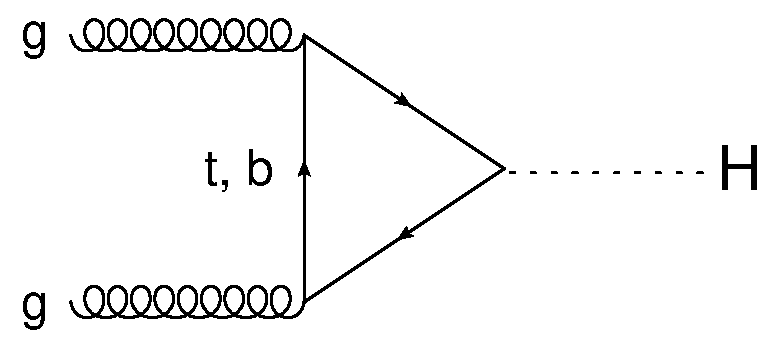
\includegraphics[width=0.4\linewidth]{T/FIGS/ggF}
			\caption{Lowest order Feynmann diagram contributing to \ggF.}
			\label{fig:ggf}
			\end{figure}
			
		\subsubsection{Vector Boson Fusion}
		
			Production of a Higgs boson from the fusion of vector bosons radiated from initial-state quarks is the second largest cross-section at the LHC, as is useful as a production mode due to topological characteristics which can distinguish the event from ggF. In VBF, the Higgs boson is produced along with two jets in the forward regions of the detector \note{Maybe need to link to the detector section}, which originate from the initial quarks as shown in Figure \ref{fig:vbf}. In addition central jet activity is suppressed due to the lack of colour exchange between quarks \cite{VBF2004}.  These distinct features mean that while the cross section for VBF at a Higgs mass of $< 200$ GeV is dominated by ggF, the easy to detect signature means the channel is a cornerstone of searches for the Higgs boson.
		
					\begin{figure}[h]
						\centering
						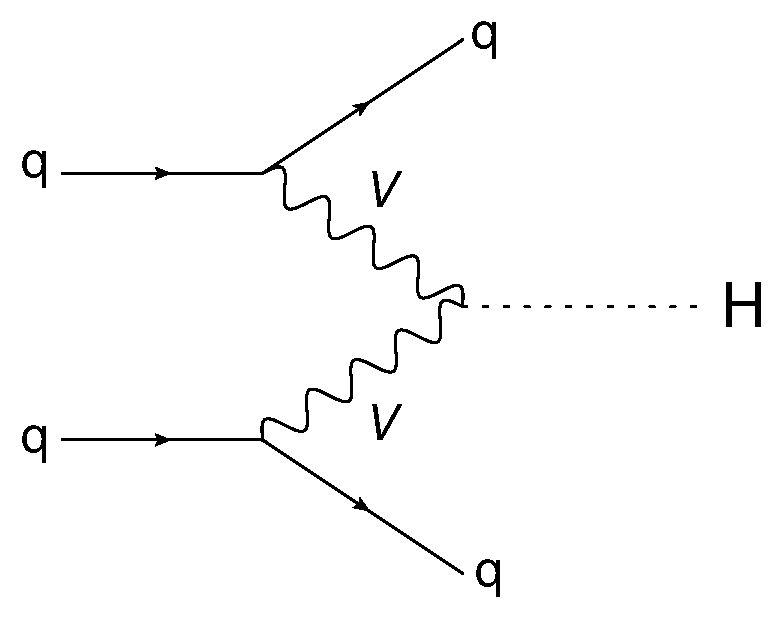
\includegraphics[width=0.4\linewidth]{T/FIGS/vbf}
						\caption{Feynmann diagram for the production of a Higgs boson via vector boson ($V$) fusion, where q denotes any quark or antiquark}
						\label{fig:vbf}
					\end{figure}
						
	\subsection{Higgs Decay} 
	
		The branching ratios for decays of the Higgs boson in the Standard Model have been extensively determined using Monte-Carlo event generators. As is to be expected, the relative cross-sections of the decay modes are strongly dependent on the mass of the Higgs boson, as highlighted in Figure \ref{fig:higgsbrlm}. 
	
		\begin{figure}[h]
			\centering
			\includegraphics[width=0.5\linewidth]{T/FIGS/Higgs_BR_LM}
			\caption{Higgs decay branching ratios for the low mass region with their uncertainties \cite{LHCHiggsXS2013}.}
			\label{fig:higgsbrlm}
		\end{figure}
		
		While observations consistent with the Standard Model Higgs boson have been made for the $H\rightarrow \gamma\gamma$, $H\rightarrow ZZ$, $H\rightarrow W^+W^-$ and $H\rightarrow \tau^+\tau^-$ channels, observation of th $H\rightarrow bb$ decay channel is significantly hindered owing to the large background from multijet production (Section \ref{T:multijer} maybe?) in hadron collisions. Despite this, the topology of the VBF production mechanism makes it a viable option for observation of the  $b\bar{b}$decay  channel.

	
	\subsection{Vector Boson Fusion}
	
	
	
	
\endinput
